\fancyhead[LO]{{\scriptsize {\FA \ }我们最幸福 {\FA } 流浪的燕子}}%奇數頁眉的左邊
\fancyhead[RO]{{\tiny{\textcolor{Gray}{\FA \ }}}\thepage}
\fancyhead[LE]{{\tiny{\textcolor{Gray}{\FA \ }}}\thepage}
\fancyhead[RE]{{\scriptsize {\FA \ }我们最幸福 {\FA } 流浪的燕子}}%偶數頁眉的右邊
\fancyfoot[LE,RO]{}
\fancyfoot[LO,CE]{}
\fancyfoot[CO,RE]{}
\chapter*{11 {\FA } 流浪的燕子}
\addcontentsline{toc}{chapter}{\hspace{5mm}11 \textbf{>}\ \ 流浪的燕子}
\vspace{5mm}
\begin{flushright}
	\textcolor{PinYinColor}{\EN \huge{Wandering\\
	Swallows\\
	\ \\}}
\end{flushright}
\begin{figure}[!htbp]
	\centering
	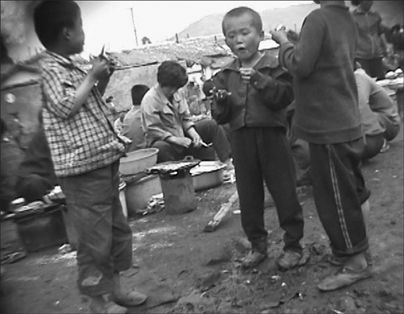
\includegraphics[width=6cm]{./Chapters/Images/11.jpg}
	\caption*{北朝鲜市场上的男孩}
\end{figure}


由于经常去清津火车站,宋女士总会与一个小男孩不期而遇,他总穿着一件很不合身的靛蓝色的工装,衣服很大下摆都盖过他的膝盖了。乱糟糟的头发里长满虱子,脚上裹着聚乙烯塑料袋而不是鞋子,看不出来又大多年纪,大概14吧,个子却和一个美国8岁的孩子差不多。\\

如果有没卖完的饼干,宋女士就会给他一些。不然,她就会从他身边走过,也不会专门去注意他。这个孩子和其它数以百计的其它在火车站流浪的孩子相比,没什么特别之处。北朝鲜人叫他们流浪的燕子(Kochebi)──这些孩子不是父母双亡的孤儿,就是父母外出找吃的,把他们落下的。他们必须要自己照顾自己,也总是一群一群的像鸽子一样,在火车站附近到处翻找可以吃的东西。在这个国家,他们是一道奇特的风景线,之前这个国家从来没有无家可归者。\\

金赫虽然个子小小,但是他很健壮也很狡猾。如果你在火车站买一点小吃,还没等送到你嘴里,他就会从你手上一把抢过来,一口就吞掉了。商贩们一般都用布把装吃的的桶子扎的紧紧的,防止小偷小摸,但是就在罩布揭开的那一刹那,他就可以撞倒桶子,然后从地上捡起吃的就跑。这些小伎俩都是在更小的时候由于缺乏食物给逼出来的。如果不是靠着这些,他可能早就饿死了。\\

金赫是怎样沦落到无家可归、在火车站流浪的历程,可以作为一个典型的案例分析,说明的北朝鲜核心阶层的每况愈下。金赫曾是个有些特权的孩子,1982年他生于一个坚定的共产主义者家庭。他的父亲在一个旨在对南韩进行渗透的军队精英部门工作。他后来被吸收加入劳动党,在军队运作的、出口鱼类和松茸以换取外汇的商社工作。金赫的家在水南区靠近他母亲工作的清津化纤厂。金赫两个月大的时候就被送到厂子里的日间看护中心同其它在职妈妈的孩子们待在一起。\\

3岁时,母亲因心脏病突然去世后,之后金赫的生活开始陷入混乱。对于母亲,他只非常迷糊的记得她的脸──他所能回忆起最早关于母亲的记忆就是葬礼上焚香的味道。金赫的父亲很快又再婚了。金赫和大他3岁的哥哥,金哲,经常因为吃的和继母起冲突。\\

这两个男孩非常调皮,还很野──而且永远饿着。他们相信继母总是给自己的女儿,他们同父异母的妹妹更多吃的。他们就去厨房偷玉米芯,拿到市场去换煮好的面条吃。后来继母把吃的都锁了起来,他们就把她的毯子偷走拿去换吃的。\\

金赫第一次从一个陌生人那里偷东西是在他10岁的时候。他从一个商贩的推车里拿了一个红豆馅的糯米饼,然后跑掉了。他的小腿抡的比小贩快,因此就让他这样得逞了。但是祸根是,这个糯米饼又甜又香太好吃了,以至于他跑回去想拿第二个。\\

金赫的父亲把他从派出所领了回来。金赫垂头丧气,泪如泉涌。回到家,父亲用皮带好好教训了他一顿,在他腿上留下一道道红印。\\

“我的孩子没人会当贼。”他父亲怒斥道。“宁可饿死也比偷好。”\\

金赫不认同这个观点。他仍然继续的偷,每次到离家更远的地方找吃的。就在清津的南边,镜城县内,有几个煤矿。煤矿再往南就是果园。金赫和他的朋友经常扒在公交车后去那里。在90年代,他几乎隔三差五就去一次。当梨子摘完了,他们就偷玉米。有一次他们被抓住,由于年纪太小,警卫只是警告了下就放他走了。金赫丝毫不为自己的偷窃行为感到羞耻。即使在金日成逝世的哀悼期,连那些为了让人们到铜像前寄托他们的哀思而准备的米糕,他都偷。\\

金赫的父亲对儿子的行为感到暴怒,但是也拿他没办法。家里也没什么吃的,以至于金赫的继母带着妹妹回了自己的娘家。此时,金赫的父亲换了工作,他当上了一家精神病看护中心的党委书记。他把儿子们安置在原来护工住的房间里。金赫很喜欢住在看护中心同病人聊天的日子。那些病人同他一样孤独,因此他们把和金赫当成大人一样和他聊天,而不是把他看成个孩子。但是看护中心食物也很短缺。虽然父亲是看护中心的党委书记,一把手,比其它的人更有权力,但是他也没有额外的食物配给。他能做的就是利用关系,把儿子们送进孤儿院。\\

同许多其它的共产党国家一样,北朝鲜的孤儿院里不只有孤儿,还有被父母遗弃的孩子。就像是全日制学校,孤儿院提供教育住宿,和膳食。能被孤儿院接收,这可是一种特权。\\

Donsong第二十四孤儿院位于稳城郡,是咸镜北道最北部的一个郡,靠近中国边界。父亲带着他们在9月的第一个星期坐火车到了那里,这样他们可以赶上新学年的开始。金赫11岁,进入小学的最后一个年级;他哥哥14岁,进入初中学习。去一趟路上要花6个小时,车上人满为患,父子们找不到座位,也一路无话。\\

“你们俩是兄弟。以后要相互照顾。不要让别人欺负你。”他们的父亲在签完放弃监护权,由孤儿院负责看护的文件后,这样对他们说。\\

当父亲往回走的时候,金赫第一次注意到父亲已经老成什么样子了。曾经高大、英俊的父亲,现在一脸憔悴,背也驼了,头发满是丝丝白发。\\

起初,孤儿院的餐厅还能勉强控制住男孩们的饥肠。当时还是秋天,收获的季节,食物很充足。男孩们很高兴每天都能有一碗米饭。即使米饭里混着玉米、大麦还有其它一些便宜的粗粮,但是这可是他们这么多年来吃的最好的东西。到了春天,他们发现孤儿院里满是树木的院子里种着杏子。他们爬上树,摘杏子吃。\\

可是在冬天,他们的食物配给被削减,孩子们只能吃到一碗只飘着几根玉米面条的咸汤。在1996年的头3个月,孤儿院死了27个孩子。金赫和他的哥哥开始旷课,到附近的镇子上找吃的。他们发现那里的状况也好不到哪里去。金赫遇见一个和他差不多大年纪的男孩,这个男孩的父母双亡,他和一个6岁的妹妹住在一起。邻居们定期会来给他们一碗粥,但也仅此而已,孩子们要自己照顾自己。\\

金赫和哥哥还有他们新交的朋友一起到处找吃的。金赫是爬树的好手,长长的手,非常有力,补偿了他那又短又粗的腿。他可以轻而易举的爬上松树,用锋利的小刀,削去外层粗糙的树皮,得到内层的嫩皮。内层嫩皮是黄色的,很有嚼劲,有点甜,有时候他还抱着树的时候就会迫不及待的开始吃了。其它人也想学他,但是金赫总能爬到更高的地方,那里的树皮没人碰过。\\

“你真像个小猴子。”他的朋友总是钦佩的说。\\

金赫又成为猎人。他猎杀老鼠,耗子,青蛙和蝌蚪。当青蛙消失了,他就抓蚱蜢和知了。在清津还很小的时候,他曾经看过朋友在水南河边抓知了吃,但是他总觉得很恶心。现在他没什么挑剔的了。他用网兜和一些东西做个了逮松鼠的机关,里面用线挂一个玉米粒作为诱饵。他们把抓到的小鸟拔毛后,用火烤着吃。他还试图用篮子和绳子来抓鸽子,但是发现鸽子非常聪明不上当。\\

狗却没那么聪明。金赫发现一只走散的狗,很小,很友好的摇着尾巴跟着他进到朋友的院子。金赫突然关上后面的门。他和朋友一起抓住它,把它塞到装满水的桶子里,盖上盖子。溺水的小狗挣扎了整整十分钟才咽气。他们把它剥了皮,烤着吃了。狗肉是朝鲜人的一种传统饮食,但是金赫很喜欢动物,事后觉得很内疚,暗下决心再也不干这样的事情了-其实到1996年中期,狗都已经很少了。\\

金赫继续偷。他和他哥哥翻墙,挖出人们埋在私人院子里的泡菜坛子。之后用手掏出泡菜直接往嘴里送。金赫始终记得他父亲的话:“宁可饿死也比偷好。”\\

有时候,金赫想象再碰到类似情况,他会反驳,“如果饿死了,没人会当你是英雄。”\\

现在,金赫很想家,他想父亲还有哥哥金哲。当16岁的时候,达到法定成人年纪后,哥哥离开了孤儿院。金赫总是依赖哥哥当自己的保镖,在童年里那些无法无天、恣意妄为的时光里,哥哥总是保护着他。金哲继承了父亲的大个子。现在哥哥离开了,金赫总是挨打。有一天,他在外面砍柴火时,遇到一伙来自稳城的男孩也在找柴火。城里的孩子经常找孤儿院孩子的茬,他们指责(正当的)孤儿院的孩子偷了他们的食物。起初,金赫以为有人朝他泼了一桶水。后来,他意识到他的脚被血浸湿了。对方用斧子在他大腿上砍了一道深深的口子。当伤口一好,他决定混上火车回清津。\\

当金赫回到清津时,他几乎都不认识自己的家乡了。清津看上去就像一个死城。所有的东西是是荒芜的、破烂的、阴郁的。商店关门歇业。火车站附近也没有公交车。他就沿着平行于海岸线的第一大街走回了家。当他穿过水南河的时候,他清楚的看到沿着海边一排的烟囱之中,没有一个冒烟。过了桥,他转向通往母亲曾经工作的那间化纤厂的大路。化工厂的大门挂着锁,里面的房子看着让人伤心。窃贼洗劫了厂里所有的机器。天慢慢黑了,当金赫到了自己家那一带时,他几乎什么都看不见。他觉得自己像是站在没有月光的旷野之中。儿时家附近一些标志性的东西,不是在他不在的时候变换了位置,就是躲在阴影之下。\\

最后,金赫还是找到了自己家的那幢楼。推开没上锁的前门,他走进了黑乎乎的楼梯间,摸索着拾级而上,一层楼、一层楼的数着。楼里是如此之安静,好像整栋楼被废弃了一样,仅仅有孩子的啼哭声,而且越往上爬,哭声就越大。他开始怀疑自己是不是弄错了。他家在第八层,从顶层向下第二层。当他走到楼上,他看见门缝下透出一缕灯光──也许是煤油灯──此时,他满心希望。\\

他敲敲门。一个年轻、漂亮怀里抱着一个婴儿的妇女开了门。她请金赫进了门,解释到她和丈夫差不多一年前从金赫父亲的手上买了这间公寓。他没有留下任何地址,但是他留有口信:“如果我的儿子们回家了,告诉他们到火车站来找我。”\\

清津火车站。只有当人们一无所有,无处可去之后才会去的容身之所。那里和完全放弃,躺在路边不同。火车的来来往往产生一种错觉,让人们对生留有一丝的希望。它让人们幻想进站的火车会带来些吃的,或者火车能带他们去好些的地方,而且他们能搭上车。清津在北朝鲜铁路网是个重要的大站──沿着海岸延伸的南北线与通往中国边境向西的铁路线在这里交汇。人们争相涌向清津,期待能找到些吃的,因为其它的城市──咸兴、吉州、金策──那里的情况更糟糕。人们不停的迁徙流动。他们还没有放弃生的希望。\\

火车站是个非常巨大的、用大理石装饰的、有着一排又高又窄窗户的两层楼建筑。屋顶上有一副巨大的金日成画像,画像的尺寸同建筑物成适当的比例。画像下面是一个石面的钟,偶尔它能报准时间。车站里,空气弥漫着火车排出的废气和香烟的烟雾。\\

人们坐在自己的腿上,空等着。如果他们太虚弱,就会席地躺在候车室或者昏暗走廊的地板上。金赫在人群中徘徊着,寻找四肢细长,走路姿势像父亲一般的人。他弯着腰,凑近了仔细看每个人的脸,希望能找到熟悉的目光。他之前的邻居很多人现在都污秽不堪的挤在火车站,但是没人知道关于他父亲和哥哥的消息。由于无处可去,金赫发现一个凹槽,那里原本是用于容纳一扇厚重铁门的。他吸了一口气,爬进凹槽处,蜷缩在里面,然后在里面美美的睡了一觉。早上,他找到个有水的水龙头,所以好好的洗了把脸,但是头上的虱子却怎么也清理不干净。\\

这里值得注意的是,在北朝鲜沦落成无家可归是很不寻常的。这是因为,毕竟,这个国家花费巨大建立了一套可以追踪自己国民的体系。每个人都有自己固定的地址,工作单位,这一切都和食品配给相挂钩──如果你离开家,你就没有吃的。人们没有旅行证都不敢去邻县去看望亲戚。即使夜里突然到访的客人都要去人民班登记,而人民班要把来访者的姓名,性别,身份证号,旅行证号,来访目的等信息一一上报给警察。警察会定期的在半夜里进行突击检查,确保没有人有未经批准的访客。每一个人时时刻刻都要带着“公民证”一本12页护照大小的本子,里面记载持有人的全面信息。那是按照苏联旧式身份证的模式制作的。\\

在饥荒中,所有都改变了。没有食物配给,没有理由再待在固定的地址了。如果坐在家就意味着会被饿死,那当局的任何恫吓都不足以把人留在家里。有史以来第一次,北朝鲜人开始在自己的国家无所顾忌的到处游荡。\\

在无家可归者之中,有异常大的比例是孩子或青少年。有些孩子的父母是外出找活干或者找吃的去了。但是还有另外一种看似非常奇怪的解释。面对这食物短缺,很多北朝鲜家庭采取了非常残酷的分配方式──他们放弃自己的食物,通常是年长的祖父母,以确保年轻一代得以存活。在这个战略下,就产生了异乎寻常多的孤儿,因为孩子们往往是整个家庭被毁灭后最后剩下来的。\\

朝鲜语Kochebi,意为流浪的燕子,站在火车站外的人群之中。就像金赫一样,他们都穿着成人尺寸的靛青色工作服,衣服看上去好像就是挂在他们身体上一样。由于工厂关门,现在工装有剩,当局有时候就把工装挂在外面,供人们免费取用。他们称之为“社会配备。”很少的孩子有鞋。如果有,他们马上就会用它换吃的,然后找几个塑料袋套在脚上。因此他们大多都有冻疮。在食品短缺的第一年,火车站的孩子靠乞讨维生,但是没过多久,他们的数量越来越大,而且也没有多少人有多余的吃的可以施设。“自己吃饱了才有余粮做慈善。”北朝鲜人都这么说;当你自己的孩子都在挨饿,你不可能去可怜其它孩子。\\

当讨不到吃的时,孩子们就在地上捡拾任何可以吃的东西。如果找不到食物,他们也会捡烟头,用废纸把剩余的烟丝卷起来。几乎每个孩子都吸烟以缓解他们的饥饿。\\

金赫有时候会加入一些孩子组成的流氓团体,一起偷东西。清津一直因其街头流氓而颇有污名,但是他们这样做也是在非常时期时,不得已而为之。也很自然的,他们分成两类:一类是大些的孩子,跑得更快些,也更强壮些;另一类是小些的孩子,这样他们被抓后不至于挨打或者被捕。大些的孩子通常会去冲撞饮食摊点,把所有的东西打翻在地。当愤怒的摊主去追他们的时候,小些的孩子就去铲取地上的食物。\\
\\

另外一个伎俩就是找到开的很慢的运送谷物的火车或卡车,用很尖的杆子捅破货物的袋子。无论漏出来什么,对每个孩子都是公平的。最后,铁路公司雇佣武装押运,而且执行射杀命令以杜绝此类盗窃。\\

他们的生活充满危险。孩子们不可能安安心心的睡觉,时时刻刻担心有人或者是另外流氓团伙会偷走他们仅有的一点东西。他们之间还流传着恐怖的故事说有专门拐骗孩子的大人。他们拐骗孩子不是为了性,而是要吃他们。金赫听说有人会给孩子下药,然后杀害他们,吃他们的肉。火车站后,靠近铁道有一些用小炉子卖汤和面条的小贩,有人说肉汤里翻滚的灰色的肉就是人肉。\\

不管是不是市井传言,吃人的说法传遍整个市场。宋女士是从和一个阿玛闲聊中听到这个故事的。\\

“不要买任何来历不明的肉。”她偷偷警告她。这个妇女声称她知道谁吃过人肉,据称味道还很好。\\

“如果你不知道,你就祈祷那是猪肉或牛肉吧。”她的这些话把宋女士吓坏了。\\

故事越传越玄乎。还有人说,一个父亲饿的精神错乱后,把自己的孩子给吃了。一个市场上的妇女据说因为卖人骨头熬成的汤而被捕。从我对脱北者的采访得知,这种情况确实发生过,而且至少有两起──一起发生在清津,一起发生在新义州,两起案件中,罪犯都被逮捕并且因为食人而被处决。然而,没有证据证明这种情况曾大规模发生,或者达到中国发生于1958年-1962年,饿死3000万人的大饥荒所记载的程度。\\

即使没有吃人现象或者其它捕食者,孩子们在街头还是活不了多久。年纪小的很难活过几个月。宋女士的大女儿,玉熙,住在火车站对面公寓楼的2楼,已经习惯每天回家的路上经过这些孩子们。\\

“这些小的可能熬不到明天早上。”玉熙会这样告诉自己,之所以这么想,部分原因是为自己做出经过这些孩子而不施以援手的决定做自我安慰式的辩护。\\

大部分我采访的清津人都提到了,在火车站和火车上散落着大量的尸体。一个工厂女工告诉我,她曾经有一次坐火车从吉州到清津,她所在的车厢里有个人就这么坐着、坐着就死了。那个人是个退伍的军官,僵硬的手指还抓着他劳动党的党员证。她说坐在旁边的人对他的死一个个都是无动于衷。她猜火车到了清津之后,尸体就被拉走了。\\

在火车站,清洁人员会定期巡视周围的公共区域,把尸体用木手推车拉走。他们会先在候车室里转转,然后再去站前广场,然后算一算地上躺着的从昨天开始就没有挪窝的人的数量。金赫说有时候他们一天要从火车站抬走多达30具的尸体。要确认他们的身份非常困难,因为没有人有身份文件,这些文件早就随好些的衣服、鞋子被偷掉了。由于这些人的家人可能已经死了或走了,这些尸体就被集体掩埋了。在儒家社会,这样处理对死者是非常不敬的,儒家思想认为祖先的坟墓所在地对子孙后代的兴旺发达有着至关重要的作用。\\

有些靠近中国边境的这样的坟墓被南韩一个叫诤友的佛教组织所见证。安德鲁纳塔索斯──一个美国援助官员也亲眼目睹了这样一个坟茔。他看见很多尸体用白色塑料纸包裹,放进墓地旁挖的一个大坑里面。之后,工人再在大坑旁,低头默哀。\\

金赫相信他父亲就被埋在这样的坟茔里面。一年后他碰到个熟人,他告诉金赫,父亲在1994年的冬天待在火车站,到了1995年,他被送进了医院。这个自傲的人,发誓从不偷窃的人,可能是第一个被饿死的人。\\

一旦放弃找到父亲的希望,金赫就没什么理由继续待在清津了。他又溜上了车。这对金赫来说很容易。在年久失修的铁轨上,火车开的很慢,而且频繁的临时停车。金赫只要跟着车跑一段距离,之后一把抓住车厢之间的把手,就用他猴子一般的手臂把自己提了上去。车厢里非常拥挤,以至于乘警无法通过走道去检查乘客的旅行证件和车票。金赫不喜欢封闭的空间,所以他爬到了车顶。车厢的顶部略带弧形,有点像面包。他在中间找了个稍平一点的地方,这样他可以平躺下来,以避开头顶上的电线。用他随时的包做枕头,他就这样一趟就是好几个小时,身体随着车厢晃动,眼睛看着头顶上飘着的白云。\\

一开始,金赫只是到了这个城市的郊区。他回到镜城,小时候他曾经在那摘梨,偷玉米。但是现在想偷更难了──农场有武装巡逻──所以金赫只有去更远的地方。他回到了位于稳城的孤儿院。现在稳城看上去不会比清津好。他记忆里孤儿院里茂密的树林,现在也被砍的差不多了。他知道离孤儿院仅仅几公里之外,从宿舍的窗户就可以看见的山脊的另外一边是一条细长如灰带一般的河──图们江──一眼望不到头。河的另外一边,那里树木仍然郁郁葱葱,玉米地也没有用枪守卫。\\

那个地方叫中国。\\

中朝两国边境沿着两条河延绵1400公里,这两条河都发源于朝鲜称为白头山,中国称为长白山的休眠火山。向南流的鸭绿江是著名的一条江,在朝鲜战争中,中国军队从此把美国军队逼了回去。中朝之间很多的官方贸易就是跨过这条江,大部分是在鸭绿江位于黄海的河口处进行的。相对于鸭绿江,图们江就仅仅比小溪宽一些,很浅,水流很缓。图们江向北流去,蜿蜒扭曲,勾勒出北朝鲜的东北边境,在海参崴的西南入海。图们江很窄,窄到即使在雨季,丰水时期,一个人很容易就可以游过去。\\

孤儿院的孩子们不允许在图们江附近玩耍。整个边境区域都是封闭的军事禁区。如果他们在图们江的支流里游泳时,太靠近边界的话,就会有边防警察把他们赶走。沙质的河岸很缓,岸边也没有什么长的够高可以提供掩护的东西。但是从稳城往南走一个或者两个小时,就是一片人烟稀少的地区,那里的河岸长有很高野草。边境守卫也离的很远,一个人很容易从这里溜过去。一般,一个边境哨位有两个人,一个人看守,一个人睡觉。但是凌晨一点一过,通常两个人都会睡着。\\

金赫第一次跨过图们江是在1997年的晚些时候。那是一个枯水期,江水的水位很低,江两岸沙质的河岸就象指尖一样几乎可以碰到一起。但是江水很冷,当金赫踏进去时,那刺骨的寒冷如同给他一记重击。虽然水深仅及他的胸膛,但是暗流不断的冲击着他的脚底。他不断的被推向下游,最终当跨过江之后,他发现自己走了一个斜线。最终当他艰难的爬上对岸时,暴露在寒冷的空气里,衣服冻得就像一件盔甲。\\

金赫之前对中国毫无兴趣,对于中国,他认为那是一个和他自己的国家一样贫穷的共产党国家。第一眼看上去的时候,中国和北朝鲜没什么区别,但是当他从河岸继续往内陆走的时候,他发现延绵数公里的已经收割过的玉米地。在一个红砖小房子里,囤有一个食槽,脱壳的玉米一直堆到了天花板,房子前面的棚架上满是南瓜和豌豆。他逛到了一个小镇上。这里比他想象的繁荣的多,有出租车、摩托车、还有人力车。商店的标牌用的是中文和朝鲜文。他很高兴的了解到,这里的很多居民虽然是中国公民,但是他们都是朝鲜族,说和自己一样的语言。他们很快就认出他是北朝鲜来的,不仅仅是因为他衣衫褴褛。15岁了,他的身高才150公分,因此相对于身体,他的脑袋就很大,这是长期营养不良的典型症状。当孩子营养不好的时候,他们的脑袋会发育成正常大小,但是身体就会矮小的多。\\

在一个市场,金赫预见一个卖碟子,首饰和小摆件的人。他问金赫能不能从北朝鲜弄些熨斗过来──那种用炭加热的老式熨斗。在北朝鲜几乎每家每户都有这样的熨斗,但是人们很少用它──特别是当衣服面料变成化纤的之后。金赫可以以几乎白给的价格在北朝鲜收到这样的熨斗,然后在中国以差不多每个10美元的价格卖掉。这可是他一辈子都没见过的、这么多的钱。带着赚到的钱,他可以回北朝鲜买更多的东西带来中国卖。瓷器、首饰、字画、玉石。他还专门买了一个Podegi,北朝鲜妇女传统的用来背孩子的布。用这块布,他把收购的东西背在背上,这样他可以带比用背包更多的东西。\\

金赫开始周期性的跨越国界。他仔细研究过边境的哨位,哪些地方的警卫心不在焉,懒惰,或者可以收买。他还发现跳进江里之前最好把衣服脱掉。他开始变得在将衣服和买的货顶在头上过江时,仍然能很熟练的保持住身体的平衡。\\

他不再偷东西。如果他想吃碗面,他就用自己的钱买一碗。他还买了裤子、一件T恤、一件蓝大衣还有一双运动鞋,这样他看上去再也不像一个难民了。他试想着就这样继续下去,掌握自己的生活。私下收购物品,并以牟利为目的进行售卖是违法的,没有旅行证件跨越国境更是罪加一等。在16岁的时候,法律上金赫成年了,从现在起,任何不当行为就会被严肃处理了。\\
